%%%%%%%%%%%%%%%%%%%%%%%%%%%%%%%%%%%%%%%%%%%%%%%%%%%%%%%%%%%%%%%%%%%%%%%%%%%
% Trim Size : 11in x 8.5in
% Text Area : 9.6in (include Runningheads) x 7in
% ws-ijbc.tex, 24 Jan 2010
% Tex file to use with ws-ijbc.cls written in Latex2E.
% The content, structure, format and layout of this style file is the
% property of World Scientific Publishing Co. Pte. Ltd.
%%%%%%%%%%%%%%%%%%%%%%%%%%%%%%%%%%%%%%%%%%%%%%%%%%%%%%%%%%%%%%%%%%%%%%%%%%%
%

%\documentclass[draft]{ws-ijbc}
\documentclass{ws-ijbc}
\usepackage{ws-rotating}     % used only when sideways tables/figures are used
\usepackage{epstopdf}
\usepackage{mathrsfs}
\usepackage{graphicx}
\usepackage{subfigure}
\bibliographystyle{ws-ijbc}

\begin{document}

\catchline{}{}{}{}{} % Publisher's Area please ignore

\markboth{Author's Name}{Paper Title}

\title{A Heteroclinic Connection between two Saddle Slow Manifolds in the Olsen Model}

\author{Elle Musoke, Bernd Krauskopf and Hinke M. Osinga}

\address{Department of Mathematics, University of Auckland, Private Bag 92019\\
Auckland, 1142, New Zealand\\
elle.musoke@auckland.ac.nz}

\maketitle

\begin{history}
\received{(to be inserted by publisher)}
\end{history}

\begin{abstract}
The abstract should summarize the context, content and conclusions
of the paper. It should not contain any references or displayed
equations. Typeset the abstract in 10~pt Times Roman with
baselineskip of 12 pt, making an indentation of 1.6~cm on the left
and right margins.
\end{abstract}

\keywords{A list of 3--5 keywords are to be supplied.}
\section{Introduction}

Slow-fast dynamical systems are characterized by a separation of variables into those that evolve on a fast time scale and those that evolve on a slower time scale.  The separation of variables into fast and slow can be found in many systems in the world around us: chemical systems, neurons, electric circuits, lasers and predator-prey dynamics have been, among others, described by slow-fast models  \cite{BZ_reaction, Neurons,Circuits, lasers, Predator-Prey}.  By reason of their ubiquity, the various phenomena that arise from the multiple-time-scale nature of slow-fast systems are of significant interest. These have been be described for two- and three-dimensional systems by well-established theory \cite{canard_explosion, lents-rapides, enlacement,singular_hopf, folded_node,three}.  Small-amplitude limit cycles transitioning to larger-amplitude relaxation oscillations were studied in two dimensions, for example, the Van der Pol oscillator and FitzHugh-Nagumo model \cite{canard_explosion, fitz-hugh-nagumo}.  In three-dimensional systems, periodic orbits with epochs of localized small-amplitude oscillations (SAOs) and epochs of large-amplitude oscillations (LAOs) have been observed \cite{BZ}.  The mechanisms that cause SAOs of these appropriately named mixed-mode oscillations (MMOs) are described in \cite{MMO}.  We now investigate novel phenomena that arise in four-dimensional slow-fast systems which may provide insight into undiscovered mechanisms for MMOs in higher dimensional systems.


We consider a prototypical four-dimensional slow-fast dynamical system that exhibits MMOs.  We study the so-called Olsen model for peroxidase-oxidase reaction, first introduced by Lars F. Olsen in 1983  \cite{Olsen}, in a parameter regime corresponding to three fast and one slow variable.  Mechanisms for MMOs in the Olsen model were previously investigated in \cite{QSSA} after an assumption was made to reduce the model to a three-dimensional system.  Manifolds on which the flow evolves on the slower timescale were computed along with the manifolds of trajectories converging to them in forward and backwards time respectively.  These gave insight into the formation of MMOs as well as the cause of their particular geometry.  However, because of the assumptions used to reduce the model to a three-dimensional system, some of the computed manifolds were of lower dimension than the corresponding manifolds in the full system.  In this research, we develop techniques for computing the same manifolds in the full four-dimensional model in the interest of studying their geometry and interactions with each other.  In particular, we focus on interactions between higher-dimensional manifolds that do not exist in systems of three dimensions or lower.


To better observe the separation between fast and slow variables, we use a change of coordinates described in \cite{Rescaling} and given by the system of ODEs
    
\begin{equation}
\begin{aligned}
\begin{cases}
\frac{dA}{dt} &= \mu - \alpha A - ABY, \\
\frac{dB}{dt} &= \varepsilon(1-BX - ABY), \\
\frac{dX}{dt} &= \frac{1}{\eta}(BX - X^2 +3ABY - \zeta X + \delta), \\
\frac{dY}{dt} &= \frac{\kappa}{\eta}(X^2 - Y - ABY),
\end{cases}
\end{aligned}
\label{equation_1}
\end{equation}
    
\noindent
where $(A, B, X, Y)\in\mathbb{R}^{4}$ are positive concentrations of chemicals.  The system parameters given by Greek letters in Table 1 are functions of original system parameters given in \cite{Olsen}. They were chosen to be the same as in \cite{Rescaling} with a minor modification.  (For notational convenience, we have substituted  $\varepsilon_{b}$ and $\varepsilon^{2}$ with $\varepsilon$ and $\eta$, respectively.)

\begin{table}[h]
\tbl{System parameters for system (1)}
{\begin{tabular}{c  c  c  c  c  c  c  c  c} \\[-2pt]
\toprule
$\alpha$ & $\delta$ & $\varepsilon$ & $\eta$ & $\kappa$ & $\mu$ & $\zeta$ \\[6pt]
\hline\\[-2pt]
0.0912 & 1.2121e-04 & 0.0037 & 0.0540 & 3.7963 & 0.9697 & 0.9847\\[1pt]
\botrule
\end{tabular}}
\end{table}

The classification of variables as either slow or fast is not straightforward for the Olsen model because the variables are not consistently slow or fast over all regions of phase space.  In fact system (\ref{equation_1}) nominally has three different time scales.  The time-scaling parameters $\varepsilon$ and $\eta$ depend on the original system parameter $k_1$.  As suggested by \cite{Rescaling}, we decrease $k_{1}$ past $0.16$ to $0.1$ so that there are only two time scales.  We study a parameter regime corresponding to three fast variables, $A, X$ and $Y$, and one slow variable, $B$.

%Background section
\section{Background}
    
In the limit as $\varepsilon \rightarrow 0$, system (\ref{equation_1}) becomes
    
\begin{equation}
\begin{aligned}
\begin{cases}
\frac{dA}{dt} &= \mu - \alpha A - ABY, \\
\frac{dX}{dt} &= \frac{1}{\eta}(BX - X^2 +3ABY - \zeta X + \delta), \\
\frac{dY}{dt} &= \frac{\kappa}{\eta}(X^2 - Y - ABY),
\end{cases}
\end{aligned}
\label{equation_2}
\end{equation}
    
\noindent
in which $B$ is a parameter.  We refer to the three-dimensional system (\ref{equation_2}) as the layer equation or the fast subsystem.  If one first performs a time rescaling, $\tau = \varepsilon t$, and then considers the limit as $\varepsilon \rightarrow 0$ the system reduces to
    
 \begin{equation}
\begin{aligned}
\begin{cases}
0 &= \mu - \alpha A - ABY, \\
\frac{dB}{d\tau} &= (1-BX - ABY), \\
0 &= \frac{1}{\eta}(BX - X^2 +3ABY - \zeta X + \delta), \\
0 &= \frac{\kappa}{\eta}(X^2 - Y - ABY),
\end{cases}
\end{aligned}
\label{equation_3}
\end{equation}
    
\noindent
which is a differential algebraic system called the slow subsystem or the reduced system. The three algebraic equations in system (\ref{equation_3}) define a one-dimensional manifold called the critical manifold, $C$.  The flow in (\ref{equation_3}) is defined by the single differential equation for $B$ and it is confined to $C$.  

The critical manifold consists of equilibria of the fast subsystem for different values of $B$. These can be linearised about and their stability determined by the $3\times3$ Jacobian matrix of (\ref{equation_2}).  Equilibria at which the Jacobian's eigenvalues all have non-zero real parts are called hyperbolic, otherwise we say that the equilibrium is non-hyperbolic.  Non-hyperbolic equilibria lying on the critical manifold correspond to local bifurcations in (\ref{equation_2}).  Near a stable MMO of interest, the critical manifold has 11 branches separated from each other by non-hyperbolic equilibria of the fast subsystem.

\begin{figure}[!t]
\begin{center}
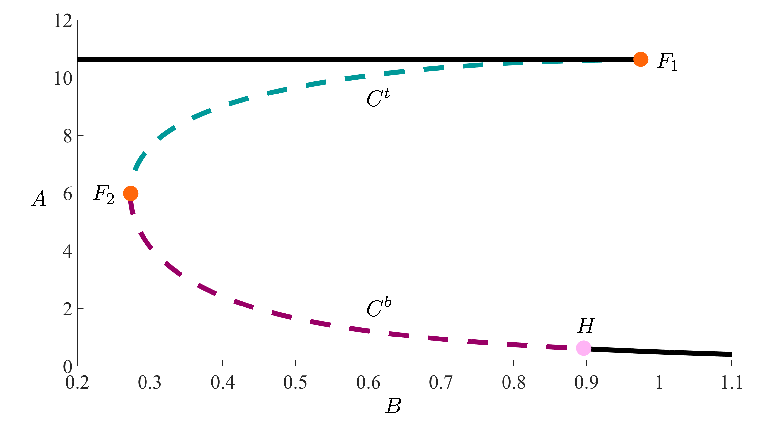
\includegraphics[page=1, width=\textwidth]{figures.pdf}
\end{center}
\caption{Physically relevant branches of the critical manifold of system (\ref{equation_1}) shown in projection onto the ($B$,$A$)-plane.  The branches labeled $C^t$ and $C^b$ and colored teal and raspberry, respectively correspond to saddle equilibria of (\ref{equation_2}), solid curves indicate stable nodes.  The two saddle-node bifurcations are represented as orange dots and labeled $F_1$ and $F_2$ respectively.  The Hopf bifurcation is represented with a light pink dot and is labeled $H$.}
\label{critical_figure}
\end{figure}

Figure \ref{critical_figure} shows four branches of $C$ on which all variables are positive projected into the ($B$,$A$)-plane.  Seven nearby branches of $C$ are not shown, because they lie in regions where at least one of $A$, $B$, $X$, or $Y$ is negative and not physically relevant.  Of the branches shown in Figure \ref{critical_figure}, the topmost black branch consists of stable equilibria of (\ref{equation_2}) and is separated from the teal-colored branch of saddle equilibria, denoted $C^t$, by a fold, shown in orange and denoted $F_1$, occurring at $B \approx 0.956$.  Equilibria $p \in C^t$ each have a two-dimensional linear stable space $E^s(p)$ and a one-dimensional linear unstable space $E^u(p)$.  The flow is from left to right near $C^t$ in the $(B,A)$-projection shown.  The fold $F_1$ has the appearance of a cusp in the ($B$,$A$)-projection, however $(B,X)$- and $(B,Y)$- projections show that this is truly a fold with respect to $B$.  Another fold, also shown in orange, separates $C^t$ from a lower raspberry-colored branch of saddle equilibria and occurs at $B \approx 0.273$ and is denoted $F_2$.  The raspberry branch of saddle equilibria is denoted $C^b$ and is separated from a branch of stable equilibria on the right by a Hopf bifurcation, represented as a pink dot and denoted $H$, occurring at $B \approx 0.897$.  Equilibria on $C^b$ have each one stable and two unstable eigenvectors.  The flow is from right to left near $C^b$.
    
We denote the local stable and unstable manifolds of points $p \in C$ by $W^{s}_{loc}(p)$ and $W^{u}_{loc}(p)$.  These are the trajectories in (\ref{equation_2}) that converge to $p$ in forwards and backwards time respectively.  The saddle branch $C^t$ has a three-dimensional local stable manifold $W^{s}_{loc}(C^t)$ and a two-dimensional local unstable manifold $W^{u}_{loc}(C^t)$ defined as
    
$$W^{s}_{loc}(C^t) = \bigcup_{p \in C^t} W^{s}_{loc}(p), \hspace{1cm} W^{u}_{loc}(C^t) = \bigcup_{p \in C^t} W^{u}_{loc}(p).$$
    
\noindent
Similarly $C^b$ has a three-dimensional local unstable manifold and a two-dimensional local stable manifold defined as
    
$$W^{s}_{loc}(C^b) = \bigcup_{p \in C^b} W^{s}_{loc}(p), \hspace{1cm} W^{u}_{loc}(C^b) = \bigcup_{p \in C^b} W^{u}_{loc}(p).$$
    
We are interested in interactions between stable and unstable manifolds of $C^t$ and $C^b$ as $\varepsilon > 0$.  Although the branches $C^t$ and $C^b$ of the critical manifold are no longer invariant for $\varepsilon > 0$, Fenichel Theory guarantees that both $C^t$ and $C^b$ persist as locally-invariant manifolds called slow manifolds, denoted $S^t$ and $S^b$, that are not unique \cite{Fenichel}. Orbit segments that lie on a slow manifold remain slow for an $O(1)$ amount of slow timescale time.  Locally invariant means that solutions can only enter or leave the manifold via its edges.  
    
We can select a unique representative $S^t$ by considering the slow manifold that remains slow for the longest amount of time.  The slow manifold $S^t$ has the same dimension as $C^t$ and, as $\varepsilon \rightarrow 0$, it converges to $C^t$.  Since equilibria of (\ref{equation_2}) lying on $C^t$ are of saddle type, $C^t$ and $S^t$ are of saddle type.  The slow manifold, $S^b$, associated with $C^b$ can be similarly defined.
    
Fenichel Theory also guarantees that $W^{s}_{loc}(C^t)$ and $W^{u}_{loc}(C^t)$ persist as locally-invariant local stable and unstable manifolds of $S^t$ \cite{Fenichel}.  We define the stable manifold of $S^t$ as a family of orbit segments, $W^s$, that have a fast approach to $S^t$ and then stay close to it for an $O(1)$ amount of time.  Similarly, we define the unstable manifold as a family of orbit segments, $W^u$, that approach $S^t$ in backward time and then stay close to it for an $O(1)$ amount of backward time.  According to Fenichel Theory, $W^s$ and $W^u$ have the same dimensions as $W^{s}_{loc}(C^t)$ and $W^{u}_{loc}(C^t)$ and lie at an $O(\varepsilon)$ distance away from them, respectively.  The manifolds $W^s$ and $W^u$ are not unique, however they can be made unique by imposing boundary conditions on the orbit segments laying on them.   We can similarly define the stable and unstable manifolds associated with $C^b$.
 
 %Saddle slow manifold section   
 \section{Computation of One-Dimensional Saddle Slow Manifolds}
    
For the computation of a one-dimensional saddle slow manifold, we follow the presentation in \cite{Saeed_Paper} of a one-dimensional saddle slow manifold for a three-dimensional system.  Here we consider only the slow manifold $S^t$ associated with $C^t$; the slow manifold $S^b$ can be found in a similar manner.
    
The precise definition of the slow manifold $S^t$ is given with respect to a closed interval $[B_{\mathrm{in}},B_{\mathrm{out}}]$ for the slow variable $B$.  The values for $B_{\mathrm{in}}$ and $B_{\mathrm{out}}$ are chosen such that the interval is contained in the interval defined by the $B$-coordinates of the two fold points $F_1$ and $F_2$.  Note that there is a segment in $C^t$ for which each point $p \in C^t$ is uniquely associated via its $B$-coordinate with a value for $B_p \in [B_{\mathrm{in}},B_{\mathrm{out}}]$.  For each $B_p \in [B_{\mathrm{in}},B_{\mathrm{out}}]$ there is a unique point $p=(p_A,p_B,p_X,p_Y) \in C^t$ such that $p_B = B_p$.  We define a solid three-sphere $D_\delta(B_p)$ in the three-dimensional subsection $\{ \begin{pmatrix} A & B & X & Y \end{pmatrix} \in \mathbb{R}^4| B=p_B\}$ that has radius $\delta$ and center $p$, given formally by

\begin{equation*}
D_\delta(B_p)=\{w \in \mathbb{R}^4 | w_B = B_p, |w-p| \leq \delta\}.
\end{equation*}
    
\noindent
The union $\mathscr{D} = \cup_{B_p \in [B_{\mathrm{in}}, B_{\mathrm{out}}]} D_\delta(B_p)$ forms a four-dimensional compact cylinder.  The radius $\delta$ is small, but it needs to be at least of $O(\varepsilon)$ to ensure that $S^t$ lies in $\mathscr{D}$.  The one-parameter family of orbit segments that enter $\mathscr{D}$ via $D_\delta(B_{\mathrm{in}})$ and exit via $D_\delta(B_{\mathrm{out}})$ are candidates for $S^t$.   We impose the additional condition that $S^t$ must have maximal integration time in $\mathscr{D}$ to select a unique candidate to represent $S^t$.  This condition may be interpreted as selecting $S^t$ such that it enters $\mathscr{D}$ via $W^s$ and exits via $W^u$.
    
The set-up is similar to the set-up described in \cite{Saeed_Paper} with the difference that $D_\delta(B_{\mathrm{in}})$ and $D_\delta(B_{\mathrm{out}})$ are three-spheres rather than two-dimensional disks and $\mathscr{D}$ is four dimensional rather than three dimensional.  Plotted in green in Figure \ref{tube_figure} is a projection of the unique representative of $S^t$.  Sketched in purple is $\mathscr{D}$ with the spheres $D_\delta(B_{\mathrm{in}})$ and $D_\delta(B_{\mathrm{out}})$ at either end.

\begin{figure}[!t]
\begin{center}
\includegraphics[page=2, width=\textwidth]{figures.pdf}
\end{center}
\caption{A visualisation of the slow manifold definition projected into the $(B,A)$-plane.  The spheres $D_\delta(B_{\mathrm{in}})$ and $D_\delta(B_{\mathrm{out}})$ are represented by purple disks at either end of a four-dimensional cylinder, also represented in purple.  A computation of the slow manifold is plotted in green and labelled $S^t$.}
\label{tube_figure}
\end{figure}

\subsection{Boundary value implementation}
    
We compute $S^t$ by setting up an appropriately defined two-point boundary-value problem (2PBVP) with the pseudo-arclength continuation package \textsc{Auto} \cite{AUTO}.  We view $S^t$ as an orbit segment $\mathbf{u} = \{\mathbf{u}(s)| 0 \leq s \leq 1 \}$ of the rescaled system


\begin{equation}
\frac{d\mathbf{u}}{ds} = TF(\mathbf{u}),
\label{equation_4}
\end{equation}
    
\noindent
where $\mathbf{u}(s) = (A(s), B(s), X(s), Y(s)) \in \mathbb{R}^4$ is the vector of chemical concentrations, $F$ is the right-hand side of (\ref{equation_1}) and $T$ is the total integration time on the fast timescale, $t=Ts$.
    
To obtain an initial solution of (\ref{equation_4}), we perform a homotopy step as follows.  First, we choose $B_{\mathrm{out}} = 0.75$ at a value that corresponds to a point $p_{\mathrm{out}} \in C^t$ close to $F_1$.  We then impose the conditions
    
\begin{equation}
\mathbf{u}(0) \in \cup_{p \in C^t} E^u(p),
\label{BC3}
\end{equation}
and
\begin{equation}
\mathbf{u}(1) \in E^s(p^t_{\mathrm{out}}),
\label{BC2}
\end{equation}
\noindent
that each impose two conditions on $\mathbf{u}(0)$ and $\mathbf{u}(1)$, respectively.  The point $p$ is then a solution to the two-point boundary-value problem defined by (\ref{equation_4})--(\ref{BC2}) with $T=0$.  We then  decrease $\mathbf{u}_B(0)$ towards $F_2$ while the total integration time increases.  The integration is stopped when $\mathbf{u}_B(0)=B_{\text{in}}=0.4$, corresponding to a point $p_{\text{out}} \in C^t$, before it reaches $F_2$.
    
We remark that $D_\delta(B_{\mathrm{in}})$ defines a three-parameter family of orbit segments with initial conditions in the sphere.  We can refine our search for orbits that enter the cylinder via $D_\delta(B_{\mathrm{in}})$ and exit it via $D_\delta(B_{\mathrm{out}})$ by observing that, because $S^t$ is of saddle type, the initial point of a candidate orbit segment must lie in a small neighborhood of $W^s$ in the sphere $D_\delta(B_{\mathrm{in}})$.  Similarly the end point must remain in a small neighborhood of $W^u$ in the sphere $D_\delta(B_{\mathrm{out}})$.
    
We define the two-dimensional plane $\Phi = \{E^u(p^t_{\mathrm{in}}) + \begin{bmatrix} 0 & 0 & 0 & B \end{bmatrix}^{T}| B \in \mathbb{R} \}$ that is transverse to $W^s \cap D_{\delta}(B_{\mathrm{in}})$ and contains $E^u(p_{\text{stop}})$.  We impose the boundary conditions
    
\begin{equation}
\mathbf{u}(0) \in \Phi
\label{BC1}
\end{equation}
    
\noindent
which impose two conditions on $\mathbf{u}(0)$.  The orbit segment resulting from the homotopy step is then a solution to the 2PBVP defined by (\ref{equation_4}), (\ref{BC2}), and (\ref{BC1}).  The total integration time $T$ is a free parameter in this 2PBVP, which means that there exists a one-parameter family of solutions.  To select a unique orbit segment from this solution family, we impose the additional condition that $T$ be locally maximal.  This will be the orbit segment which locally has the longest slow segment in the geometric sense and will be the best approximation of $S^t$.  In the case where there are two such candidates, we choose one.
    
In the final continuation run we increase the integration time until a fold in $T$ is detected.  The resulting orbit segment approximates the saddle slow manifold, $S^t$.
   
A projection of $S^t$ into the $(B,A)$-plane is shown as the green curve in Figure \ref{tube_figure}.  A keen observer will note that, near $D_\delta(B_{\mathrm{in}})$, $S^t$ includes a segment of sharp decrease mostly in the $A$-direction.  This is due to the final step in our computation, where we restrict $\mathbf{u}(0)$ to move in the plane $\Phi$.  In order to increase the integration time, $\mathbf{u}(0)$ then moves toward the one-dimensional $W^s \cap \Sigma$ while $\mathbf{u}(1)$ moves toward the point $W^u \cap E^s(p^t_{\mathrm{out}})$.  The fold in $T$ signals that maximal integration time is reached and $\mathbf{u}(0)$ and $\mathbf{u}(1)$ are near respective intersection points. The result is an orbit segment containing a slow segment between two fast segments near $W^s$ and $W^u$ respectively.  In Figure \ref{tube_figure}, the segment lying near $W^u$ is so short that it is not visible.  We obtain an approximation of $S^t$ that does not include fast segments by restricting the orbit segment further within the interval $[B_{\mathrm{in}},B_{\mathrm{out}}]$.
   
The computation of the slow manifold $S^b$ associated with $C^b$ presents some extra challenges due to a saddle equilibrium of the full system lying on $C^b$ at $B \approx 0.323$ and the Hopf bifurcation of the fast subsystem at $B \approx 0.897$.  The saddle equilibrium causes a change in the direction of the flow near $C^b$ which causes a locus of points in $\mathscr{D}(B_{\mathrm{out}})$ at which the flow is tangent to the sphere for $\Delta$ sufficiently large.  It is important to note that the locus of tangency points approaches $C^b$ as $B$ decreases toward the $B$-coordinate value of $F_1$.  Orbit segments in the region of $C^b$ may also increase in integration time by including segments that follow the nearby stable slow manifold further in backwards time.  These problematic segments may be inside or outside the tube $\cup_{B \in [B_{\mathrm{in}},B_{\mathrm{out}}]}\mathscr{D}(B)$ depending on our choice of $B_{\mathrm{in}}$ and $B_{\mathrm{out}}$.  In order to overcome these difficulties, boundary conditions need to be chosen carefully to ensure that an increase in integration time results only from an approach to a saddle slow manifold $S^b$.  To this end, we follow the steps for computing $S^t$ while making necessary modifications to boundary conditions.

We begin by choosing $B_{\mathrm{in}} = 0.35$ slightly larger than the $B$-coordinate value of the saddle equilibrium of the full system and choosing $B_{\mathrm{out}}=1.0 > H_B$.  We select the unique point $p^* \in C^b$ such that $p^*_B = 0.45$.  We denote by $\phi_{\textsc{hom}}$ the plane passing through $p^*$ spanned by the real and imaginary parts of the complex conjugate eigenvectors of the stable equilibrium of the fast subsystem at $B=1.0$.  The plane $\phi_{\textsc{hom}}$ is transverse to $W^s(p^*)$ because the complex conjugate eigenvectors at $B=1.0$ change stability as the stable fast-subsystem equilibrium passes through the Hopf bifurcation with decreasing $B$.  For this reason, they are perturbations of the vectors spanning $E^u(p^*)$ which is transverse to $W^s(p^*)$.  We also define the two-dimensional section $\Gamma = \{ w \in \mathbb{R}^4 | w_A=p^*_A, w_Y=p^*_Y \}$.  A homotopy step is performed by imposing the boundary conditions

\begin{equation}
\mathbf{u}(0) \in \phi_{\textsc{hom1}},
\label{BC_unstable1}
\end{equation}

and

\begin{equation}
\mathbf{u}(1) \in \Gamma
\label{BC_unstable2}
\end{equation}

\noindent
which impose two conditions on $\mathbf{u}(0)$ and $\mathbf{u}(1)$ respectively.  The point $p^*$ is then a solution to the 2PBVP defined by (\ref{equation_4}), (\ref{BC_unstable1}), and (\ref{BC_unstable2}).  We then increase $T$ until $\mathbf{u}(1)$ attains a Euclidean distance of $0.1$ from the intersection of $C^b$ with the three-dimensional $B = \mathbf{u}_B(1)$ section.  This occurs when $ \mathbf{u}_B(1) \approx 0.437$ corresponding to the point $\bar{p} \in C^b$.  Keeping $\mathbf{u}(1)$ at a Euclidean distance of $0.1$ rom the intersection of $C^b$ with the three-dimensional $B = \mathbf{u}_B(1)$ section ensures that $\mathbf{u}(1)$ remains in a region of $\cup_{B \in [B_{\mathrm{in}}, B_{\mathrm{out}}]}\mathscr{D}(B)$ where the flow is from right to left in the $(B,A)$-projection.  The resulting orbit segment has a fast approach to $C^b$ at $B=0.45$ and remains $O(\epsilon)$ close to it for an $O(1)$ amount of slow time before making a fast exit from $\cup_{B\in[B_{\textsc{in}}, B_{\textsc{out}}]} \mathscr{D}(B)$ at $B=0.437$.

A second homotopy step is performed to extend $\mathbf{u}(t)$ backwards in time past $H$.  We define a one-dimensional circle $l = \{w \in \mathbb{R}^4 | w_B \approx 0.437, w_Y =p^*_Y, |w-\bar{p}| = 0.1\}$ and the three-dimensional $\phi_{\textsc{hom2}} = \{\phi_{\textsc{hom1}} + \begin{bmatrix} 0 & B & 0 & 0 \end{bmatrix}^{T}| B \in \mathbb{R} \}$.  We perform a second homotopy step by imposing the boundary conditions

\begin{equation}
\mathbf{u}(0) \in \phi_{\textsc{hom2}},
\label{BC_unstable3}
\end{equation}

and

\begin{equation}
\mathbf{u}(1) \in l.
\label{BC_unstable4}
\end{equation}
\noindent
The orbit segment $\mathbf{u}(t)$ obtained from the first homotopy step is then a solution to the 2PBVP defined by (\ref{equation_4}), (\ref{BC_unstable3}), and (\ref{BC_unstable4}).  In the second homotopy step, we increase integration time while $\mathbf{u}(0)_B$ increases.  The continuation is stopped when $\mathbf{u}(0)_B=1.0$.  The resulting orbit segment has a fast approach to the stable slow manifold at $B=1.0$ before passing $H$ and remaining close to $C^b$ until its fast exit at $B \approx 0.437$.  

In the next step, we aim to find the orbit segment that has the highest integration time in the tube $\cup_{b\in[B_{\textsc{in}}, \approx 0.437]} \mathscr{D}(B)$.  We define the two-dimensional plane $\phi = \phi_{\textsc{hom2}} \cap \{w \in \mathbb{R}^4 | w_B=1.0 \}$ and the two-dimensional sphere  $\mathscr{D} = \{w \in \mathbb{R}^4 | w_B \approx 0.437, |w-\bar{p}| = 0.1\}$.  We impose the boundary conditions

\begin{equation}
\mathbf{u}(0) \in \phi,
\label{BC_unstable5}
\end{equation}

and

\begin{equation}
\mathbf{u}(1) \in D
\label{BC_unstable6}
\end{equation}
\noindent
which each impose two conditions on $\mathbf{u}(0)$ and $\mathbf{u}(1)$ respectively.  The orbit segment resulting from the second homotopy step is a solution to the 2PBVP defined by (\ref{equation_4}), (\ref{BC_unstable5}), and (\ref{BC_unstable6}).  Keeping the $\mathbf{u}(1)$ close to $C^b$ in the $B \approx 0.437$ section ensures that $\mathbf{u}(1)$ does not encounter a change in direction of the flow caused by the saddle equilibrium of the full system.  Maximal integration then corresponds to the orbit segment that remains slow for the longest amount of time inside $\cup_{b\in[B_{\textsc{in}}, \approx 0.437]} \mathscr{D}(B)$.  The integration time is increased until a fold in $T$ corresponding to maximal integration time is detected.

Finally, to we perform a final homotopy step to obtain the orbit segment $S^b$ that enters $\cup_{b\in[B_{\mathrm{in}}, B_{\mathrm{out}}]} \mathscr{D}(B)$ at $B_{\mathrm{in}}$ and exits at $B_{\mathrm{out}}$.  We impose the boundary condition

\begin{equation}
\mathbf{u}(1) \in \cup_{p \in C^b}\{w \in \mathbb{R}^4 | |w-p| = 0.1\},
\label{BC_unstable7}
\end{equation}

\noindent
and continue the fold in $T$ with decreasing $\mathbf{u}_B(1)$.  The continuation is stopped when $\mathbf{u}_B(1) = B_{\textsc{in}}$.

\begin{figure}[!t]
\begin{center}
\includegraphics[page=14, width=\textwidth]{figures.pdf}
\end{center}
\caption{A computation $S^b$ is projected into the $(B,A)$-plane in green.  A segment of $C^b$ is plotted as a raspberry dotted line.  The stable branch of the critical manifold near $C^b$ is plotted in black.}
\label{tube_figure_unstable}
\end{figure}

A projection of $S^b$ into the $(B,A)$-plane is plotted in green in Figure \ref{tube_figure_unstable}.  The orbit segment includes a portion of the stable slow manifold to the right of the $H$ as well as a portion of the unstable manifold of $S^b$.  To obtain an orbit segment that only includes segments of the saddle slow manifold associated with $C^b$, we can restrict the orbit segment further inside the interval $[B_{\mathrm{in}},B_{\mathrm{out}}]$.


%Stable Manifold of Slow Manifold
\section{The Stable Manifold of a Slow Manifold}

Fenichel theory guarantees that each slow manifold $S^t$, associated with $C^t$, has a local, two-dimensional unstable manifold $W_{\mathrm{loc}}^u$ \cite{Fenichel}.  By definition, such an unstable manifold consists of a one-parameter family of orbit segments that have a fast approach to $S^t$ in backward time before remaining $O(\varepsilon)$ close for $O(1)$ (backward) slow time.  However, the unstable manifold of a saddle slow manifold is not unique and we consider only a specific candidate $W_{\mathrm{loc}}^u$ from this non-unique family of manifolds that all lie exponentially close to each other \cite{Fenichel}.  Similarly there exists a local, non-unique, three-dimensional stable manifold $W^s_{\mathrm{loc}}(S^t)$, which is defined as a two-parameter family of orbit segments that have a fast approach to $S^t$ in forward time before remaining $O(\varepsilon)$ close for $O(1)$ slow time.  The global unstable and stable manifolds $W^u$ and $W^s$ can be obtained from extending $W^u_{\mathrm{loc}}$ and $W^s_{\mathrm{loc}}$ in backward and forward time, respectively.  In the lower-dimensional model considered in \cite{QSSA}, $W^s$ was two-dimensional and computed in the region between $C^t$ and $C^b$.  We now turn to the computation of the three-dimensional manifold in the same region in the full system.
    
As $W^s$ is three-dimensional it is cumbersome to compute and difficult to visualise.  A natural way forward is to study a subset of $W^s$ as a one-parameter family of two-dimensional slices.  These can be visualised and computed with the pseudo-arclength continuation package \textsc{Auto} \cite{AUTO}.  We begin by defining a two-dimensional plane $\Sigma$ given by fixed values of $A$ and either $X$ or $Y$.  We approximate a slice with a smooth, one-parameter family of $\mathbf{u}$ that begin in $\Sigma$, enter $\mathscr{D}$ at $D_{\delta}(B_p)$ for some $B_p \in [B_{\text{in}}, B_{\text{out}}]$, and remain inside $\mathscr{D}$ for $O(1)$ slow time.  We use $W^{s}_{\Sigma}$ to denote such an approximation.  The slice $W^{s}_{\Sigma}$ is taken to be the portions of the $\mathbf{u}$ that enter $\mathscr{D}$ in the fast direction.  The portions that evolve mostly in the $B$-direction inside $\mathscr{D}$ for $O(1)$ slow time are considered to be part of $S^t$.  If a $\mathbf{u}$ includes a portion that has a fast exit from $\mathscr{D}$, that portion is considered as an approximation of an orbit segment lying on $W^u$.
    
\subsection{Boundary value problem implementation}

\begin{figure}[h]
\centering
\subfigure[A sketch of the first homotopy step in the algorithm for computing $W^{s}_{\Sigma^*}$.  A projection of $\Sigma^*$ is represented as a pink line in the $(B, A)$-plane.  The linear stable space $E^s(p_{\mathrm{out}})$ is represented by a blue cross while a sketch of $S^t$ is shown in green.]{\label{step1}\includegraphics[width=0.49\textwidth, page=3]{figures.pdf}}
\subfigure[A representative orbit segment in the first homotopy step is represented as a black curve.  Fast segments are represented with double arrows while slow segments are represented with single arrows.]{\label{step2}\includegraphics[width=0.49\textwidth, page=4]{figures.pdf}}
\subfigure[A sketch illustrating the selection of an orbit segment with maximal integration time.  Represented by a blue cube is the space $\Omega$.  The curve $\mathscr{L}$ is represented in yellow.]{\label{step3}\includegraphics[width=0.49\textwidth, page=5]{figures.pdf}}
\subfigure[A sketch of the selection of a different slice $W^{s}_{\Sigma}$.  This representation shows a selection of $\Sigma$ on the other side of the critical manifold from $\Sigma^*$ in the $(B, A)$-projection.]{\label{step4}\includegraphics[width=0.49\textwidth, page=6]{figures.pdf}}
\caption{Set up for the computation of $W^{s}_{\Sigma}$.}
\end{figure}
    
We are interested in the geometry of $W^{s}_{\Sigma}$ in the region between $C^t$ and $C^b$ where $W^s$ was found in \cite{QSSA}.  We define the plane $\Sigma^*$, given by fixing $A\approx10.6055$ and $Y\approx2.3001 \times 10^{-4}$, and compute $W^{s}_{\Sigma^*}$ by adapting a technique outlined in \cite{Saeed_Paper} for two-dimensional stable manifolds in three-dimensional systems.  We then explain the computation of $W^{s}_{\Sigma}$ for an arbitrary $\Sigma$ that is transverse to the flow and $\bigcup_{p \in C^t} E^u(p)$ in our region of interest.
    
We first perform a homotopy step by choosing $B_{\mathrm{out}} = 0.9$ corresponding to the point $p_{\text{out}}\approx[10.6055, 0.9, 4.9248 \times 10^{-2}, 2.3001 \times 10^{-4}]$.  Following the definition for $W^s_{\Sigma^*}(S^t)$, we impose the boundary condition
    
\begin{equation}
\mathbf{u}(0) \in \Sigma^*
\label{BC6}
\end{equation}
    
 \noindent
that imposes two conditions on $\mathbf{u}(0)$ since $\Sigma^*$ is two dimensional.  As part of selecting a $\mathbf{u}$ that remains close to $S^t$ for $O(1)$ slow time, we consider the two-dimensional $E^s(p^t_{\text{out}})$ that is transverse to $W^u$.  We impose the boundary condition
    
\begin{equation}
\mathbf{u}(1) \in E^s(p^t_{\text{out}})
\label{BC7}
\end{equation}
    
\noindent
that imposes two conditions on $\mathbf{u}(1)$ and allows for the possibility of $\mathbf{u}(1)$ intersecting $W^u$.  The point $p_{\text{out}}$ is a solution to the 2PBVP defined by (\ref{equation_4}), (\ref{BC6}) and (\ref{BC7}) with $T=0$.  Figure \ref{step1} illustrates an example of the set up for this homotopy step.  The plane $\Sigma^*$ is represented by a pink line, $E^s(p^t_{\mathrm{out}})$ is represented by a blue cross, and a curve representing $S^t$ is sketched in neon green.
    
We increase $T$ while allowing $\mathbf{u}_{B}(0)$ to decrease towards $F_2$.  This step is illustrated in Figure \ref{step2} where an intermediate orbit is represented as a black curve with the fast segment indicated with double arrows and the slow segment indicated with a single arrow.  The continuation is stopped at $\mathbf{u}(0)_B = B_{\text{in}}=2.3 \times 10^{-1}$, just before it reaches the $B$-coordinate of $F_2$.  A sketch of the resulting orbit segment is shown in Figure \ref{step3}.
    
The orbit segment illustrated in Figure \ref{step3} belongs to a two-parameter family of $\mathbf{u}$ that satisfy the boundary conditions (\ref{BC6}) and (\ref{BC7}).  To select a one-parameter family of orbit segments from these, we define the curve $\mathscr{L} = \Sigma^*\cap \{ \begin{pmatrix} A & B & X & Y \end{pmatrix} \in \mathbb{R}^4 | B = B_{\text{stop}}\}$ and impose the condition
    
    
\begin{equation}
\mathbf{u}(0) \in \mathscr{L}
\label{BCSTOP}
\end{equation}
    
\noindent
which imposes three conditions on $\mathbf{u}(0)$ and is more restrictive than (\ref{BC6}).  The boundary condition (\ref{BCSTOP}) is represented as a yellow line in Figure \ref{step3}.  We define the three-dimensional space $\Omega$ spanned by the two stable eigenvectors of $p_{\text{out}}$ and the vector parallel to the $B$-direction.  Note that $\Omega$ is transverse to $\cup_{p \in C^t}E^u(p)$ and hence $W^u$.  We impose the condition
    
\begin{equation}
\mathbf{u}(1) \in \Omega,
\label{BC11}
\end{equation}
    
\noindent
which imposes one condition on $\mathbf{u}(0)$ and is less restrictive than (\ref{BC7}).  Condition (\ref{BC11}) is represented in Figure \ref{step3} as a cube with dark blue edges.  The integration time $T$ is then increased forcing $\mathbf{u}(0)$ to approach $W^s \cap \Sigma^*$ and $\mathbf{u}(1)$ to approach $W^u \cap \Omega$. When a fold in $T$ is reached $\mathbf{u}(0)$ and $\mathbf{u}(1)$ have intersected $W^s$ and $W^u$, respectively and maximum integration time is attained.  
    
The orbit segment that is obtained begins in $\Sigma^*$ and has a fast approach to $S^t$ before remaining $O(\varepsilon)$ close for $O(1)$ slow time and so it lies on $W^{s}_{\Sigma^*}$ by definition.  The final step is to continue the fold in $T$ while allowing $u(0)_B$ to increase to obtain the rest of $W^{s}_{\Sigma^*}$.  

\begin{figure}[h]
\centering
\subfigure[]{\label{piece_BAX}\includegraphics[width=0.49\textwidth, page=7]{figures.pdf}}
\subfigure[]{\label{piece_BAY}\includegraphics[width=0.49\textwidth, page=8]{figures.pdf}}
\caption{The slice $W^{s}_{\Sigma^*}$, represented in blue, projected into $(B,A,X)$-space (a) and $(B,A,Y)$-space (b) with a representative orbit segment plotted in magenta.  Projections of the critical manifold are shown in black and the view is rotated relative to previous figures.}
\label{piece}
\end{figure}
   
Figure \ref{piece} shows two projections of $W^s_{\Sigma^*}$.  Although the manifold is two dimensional, it is necessary to visualise it in both the $(B,A,X)$- and $(B,A,Y)$-projections because it exists in four-dimensional space.  Lying on $W^s_{\Sigma^*}$ is a representative orbit segment, plotted in magenta.  The critical manifold is plotted in black.  The view rotated relative to other figures to help illustrate the geometry of the slice.  Orbits lying on $W^s_{\Sigma^*}$ have a fast approach to $S^t$ in $X$ and $Y$ before approaching mainly in the $A$-direction and then finally remaining close for $O(1)$ slow time.
    
In the case where we would like to compute $W^{s}_{\Sigma}$ for a different $\Sigma$, given by constant values of $A$ and $Y$ (respectively $X$), we must perform a second homotopy step after the first.  Using the orbit segment represented in Figure \ref{step3} as a starting point, we impose (\ref{BC7}) while keeping as free parameters $T$, $\mathbf{u}_B(0)$, $\mathbf{u}_X(0)$ (respectively $\mathbf{u}_Y(0)$).  In two runs, we continue $\mathbf{u}$ with $\mathbf{u}_A(0)$ and $\mathbf{u}(0)_Y$ (respectively $\mathbf{u}(0)_X$) as main continuation parameters.  In each of these runs, we increase or decrease the main continuation parameter until it attains the value necessary for $\mathbf{u}(0) \in \Sigma$.  Once $\mathbf{u}(0) \in \Sigma$, we follow the rest of the procedure above while considering $\Sigma$ instead of $\Sigma^*$.
    
Figure \ref{step4} illustrates a choice of $\Sigma$ on the opposite side of the critical manifold from $\Sigma^*$ in the $(B,A)$-projection.  The orbit segment resulting from the second homotopy step is represented as a black curve.  Conditions (\ref{BCSTOP}) and (\ref{BC11}) are again illustrated with a yellow line and a cube with dark blue edges, respectively.
    
Figure \ref{pieces} shows $W^s_{\Sigma^*}$ and four slices $W^{s}_{\Sigma}$ of $W^{s}$.  Here $\Sigma$ were selected as follows, $A\approx10.6055$ and $Y\approx2.3001 \times 10^{-4}$, $A=2.0$ and $Y\approx2.3001 \times 10^{-4}$, $A=4.0$ and $X=0.75$, $A=4.0$ and $Y=0.75$, $A=6.0$ and $X=0.5$.  The slices appear to self-intersect in each projection, however they do not do so in the full four-dimensional space.  

\begin{figure}[h]
\centering
\subfigure[]{\label{pieces_BAX}\includegraphics[width=0.49\textwidth, page=9]{figures.pdf}}
\subfigure[]{\label{pieces_BAY}\includegraphics[width=0.49\textwidth, page=10]{figures.pdf}}
\caption{A variety of submanifolds of $W^{\mathbf{s}}(S^t)$, represented in blue, projected into $(B,A,X)$-space (a) and $(B,A,Y)$-space (b) with example orbit segments plotted in magenta.  Projections of the critical manifold are shown in black and the view is rotated relative to previous figures.}
\label{pieces}
\end{figure}
    
We note that, unlike the stable manifold of $S^t$ computed in \cite{QSSA}, each $W^{s}_{\Sigma}$ in Figure \ref{pieces} diverges backwards in time in the $X$- and $Y$- directions before reaching $C^b$.  As an approximation of $W^s$, the stable manifold in the three-dimensional system suggests that there exists a $W^{s}_{\Sigma}$ in the four-dimensional system that spirals around $S^b$ in backward time for an appropriate choice of $\Sigma$.  Such a surface would be the intersection of the two three-dimensional manifolds $W^s$ and $W^u$ in the full four-dimensional system.  As two three-dimensional objects intersect generically in a two-dimensional surface in four-dimensional space, this heteroclinic connection between $S^t$ and $S^b$ would most likely be two dimensional.  Such an object would indeed be a novel phenomenon that does not occur in lower-dimensional systems.

\begin{figure}[ht]
\centering
\subfigure[]{\label{piece_BAX_unstable}\includegraphics[width=0.49\textwidth, page=15]{figures.pdf}}
\subfigure[]{\label{piece_BAY_unstable}\includegraphics[width=0.49\textwidth, page=16]{figures.pdf}}
\caption{The slice $W^u_{r^*}$ of $W^u$ is represented in red, projected into $(B,A,X)$-space (a) and $(B,A,Y)$-space (b) with example orbit segments plotted in forest green.  Projections of the critical manifold are shown in black and the view is rotated relative to previous figures.}
\label{pieces}
\end{figure}

In the computation of slices of the three-dimensional unstable manifold $W^u$ associated with $S^b$, we encounter the same complications as in the computation of $S^b$.  We modify the steps for computing two-dimensional slices of $W^s$ associated with $S^t$ in order to ensure that an increase in integration time results only from a more accurate approximation of a slice of $W^u$ associated with $S^b$.  We begin by defining for each $B_p \in [B_{\mathrm{in}}, B_{\mathrm{out}}]$ a two-dimensional sphere

\begin{equation*}
\bar{D}_r(B_p)=\{w \in \mathbb{R}^4 | w_B = B_p, |w-p| = r\}
\end{equation*}

where $p \in C^b$ is the unique point such that $p_B = B_p$.  We can then define the three-dimensional cylinder $\mathscr{R} = \cup_{B \in [B_{\mathrm{in}}, B_{\mathrm{out}}]}\bar{D}_r(B)$.  A slice $W^u_r$ is defined as a smooth, one parameter family of orbit segments $\mathbf{u}$ that enter $\mathscr{D}$ at $D_\delta(B_{in})$ and exit at $B_p \in (B_{\mathrm{in}}, B_{\mathrm{out}})$ before intersecting $\mathscr{R}$.  In the following steps, the computation of a slice $W^u_{r^*}$ is outlined for $r^*=0.7$ before the description of the necessary modifications to obtain $W^u_r$ for more general $r$. 

We perform an initial homotopy step to obtain an orbit segment that enters $\mathscr{D}$ at $B_{\mathrm{in}}$ and intersects $\mathscr{R}$ after exiting $\mathscr{D}$ at some $B^* \in (B_{\mathrm{in}}, B_{\mathrm{out}})$.  We select the unique point $p^* \in C^b$ such that $p^*_B=0.7$.  The plane $\bar{\Sigma}$ is defined by fixing the $A$- and $Y$- coordinates of $p^*$.  We impose the boundary conditions

\begin{equation}
\mathbf{u}(0) \in E^u(p^*),
\label{BC1_unstable}
\end{equation}

and 

\begin{equation}
\mathbf{u}(1) \in \bar{\Sigma}
\label{BC2_unstable}
\end{equation}
\noindent
which each impose two conditions on $\mathbf{u}(0)$ and $\mathbf{u}(1)$ respectively.  The point $p^*$ is then a solution to the 2PBVP defined by (\ref{equation_4}), (\ref{BC1_unstable}), and (\ref{BC2_unstable}) for $T=0$.  We increase $T$ while $\mathbf{u}(0)_B$ decreases and stop the continuation when $\mathbf{u}(1)$ intersects $\mathscr{R}$.  We denote by $B_{\mathrm{stop}}$ the $B$-value of $\mathbf{u}(1)$ at the end of this step.

In the second homotopy step we define a three-dimensional space $\phi_{\textsc{hom2}} = \{E^u(p^*) + \begin{bmatrix} 0 & B & 0 & 0 \end{bmatrix}^{T}| B \in \mathbb{R} \}$ and a one-dimensional circle $\mathscr{L} = \{ w \in \mathbb{R}^4 | w_Y=p^*_Y, w_B=B_{\mathrm{stop}}, |w-p^{\mathrm{stop}}|=0.7\}$ where $p^{\mathrm{stop}} \in C^b$ is the unique point such that $p^{\mathrm{stop}} = B_{\mathrm{stop}}$.  We then impose the boundary conditions

\begin{equation}
\mathbf{u}(0) \in \phi_{\textsc{hom2}},
\label{BC3_unstable}
\end{equation}

and 

\begin{equation}
\mathbf{u}(1) \in \mathscr{L}.
\label{BC4_unstable}
\end{equation}
\noindent
Condition (\ref{BC3_unstable}) imposes one condition on $\mathbf{u}(0)$ while condition (\ref{BC4_unstable}) imposes three conditions on $\mathbf{u}(1)$.  The orbit segment resulting from the first homotopy step is a solution to the 2PBVP defined by (\ref{equation_4}), (\ref{BC3_unstable}), and (\ref{BC4_unstable}).  We continue the orbit segment by increasing $T$ while $\mathbf{u}(0)_B$ increases.  The continuation is stopped when $\mathbf{u}(0)_B = B_{\mathrm{in}}=1.0$.

We define the plane $\Phi = \{w \in \phi_{\textsc{hom2}}| w_B=B_{\mathrm{in}}\}$ and impose the boundary conditions

\begin{equation}
\mathbf{u}(0) \in \Phi,
\label{BC5_unstable}
\end{equation}

and 

\begin{equation}
\mathbf{u}(1) \in \mathscr{R} \cap \{ w \in \mathbb{R}^4 | w_B=B_{\mathrm{stop}}\}
\label{BC6_unstable}
\end{equation}
\noindent
which impose two conditions on $\mathbf{u}(0)$ and $\mathbf{u}(1)$ respectively.  The orbit segment resulting from the second homotopy step is a solution to the 2PBVP defined by (\ref{equation_4}), (\ref{BC5_unstable}), and (\ref{BC6_unstable}).  Our aim is to select a smooth one-parameter family of orbit segments from the two-parameter family of orbit segments satisfying (\ref{BC5_unstable}) and (\ref{BC6_unstable}). % To this end, for each $B_p \in [B_{\mathrm{in}},B_{\mathrm{out}}]$, we select from the one-parameter family of orbit segments exiting $\mathscr{D}$ at $B_p$ the orbit segment with maximal integration time.  To find an initial orbit of this description we increase $T$ again until maximal integration time is reached.  This is detected as a fold in $T$.  Finally to obtain the rest of the slice $W^u_{r^*}$ we switch the endpoint boundary condition to

\begin{equation}
\mathbf{u}(1) \in \mathscr{R}
\label{BC7_unstable}
\end{equation}
\noindent
which imposes one condition on $\mathbf{u}(1)$.  In two runs, the fold in $T$ is continued until $\mathbf{u}(0)_B=B_{\mathrm{out}}$ and then again until $\mathbf{u}(0)_B=B_{\mathrm{in}}$ to sweep out $W^u_{r^*}$.

We can compute a different slice $W^u_r$ by returning to the second homotopy step in our computation.   Depending on the magnitude of $r$, we may need to perform one or two additional homotopy steps.  In the case where $r$ is large enough that $D^*_r(\mathbf{u}(1)_B)$ contains a locus of points at which the flow is tangent to it, an extra homotopy step is needed.  We define a plane $\phi_{\mathrm{hom3}}$ by fixing the $A$- and $X$-coordinates of $\mathbf{u}(1)$ after the second homotopy step.  The orbit is continued with the boundary conditions (\ref{BC5_unstable}) and

\begin{equation}
\mathbf{u}(1) \in \phi_{\mathrm{hom3}},
\label{BC8_unstable}
\end{equation}
\noindent
which imposes two conditions on $\mathbf{u}(1)$.  The endpoint $B$-coordinate $\mathbf{u}(1)_B$ is increased until $D^*_r(\mathbf{u}(1)_B)$ no longer contains a locus of tangent points.

The final homotopy step involves defining another plane $\phi_{\mathrm{homfinal}}$ by fixing the $B$- and $X$- values of $\mathbf{u}(1)$.  Condition (\ref{BC5_unstable}) is imposed while a new restriction

\begin{equation}
\mathbf{u}(1) \in \phi_{\mathrm{homfinal}},
\label{BC9_unstable}
\end{equation}
\noindent
imposes two conditions on $\mathbf{u}(1)$.  The radius $r$ is then increased or decreased until the desired magnitude is attained.  All that remains is to follow through with the rest of the steps to compute $W^u_r$.


\newpage
\bibliography{sample}

\end{document}
